\documentclass[11pt]{jarticle}
\usepackage[top=20truemm,bottom=20truemm,left=10truemm,right=10truemm]{geometry}
\usepackage[dvipdfmx]{graphicx}
\usepackage{ascmac}
\usepackage{url}

\title{実験D:CPA研修}
\author{}
\date{2019/8/30}

\begin{document}
\newgeometry{top=10truemm,bottom=20truemm,left=10truemm,right=10truemm}
\maketitle
\section{本研修の目的}
CPA (Correlation Power Analysis , 相関電力解析) は,暗号モジュールにおいて暗号化処理時に消費される電力と,処理から推定した消費電力の相関により秘密鍵を解析する解析手法である.
バイトごとに鍵を推定することができるため,鍵の探索空間を大きく減らすことができるなどの利点がある.
本研修では AES-128 (鍵長が128bitのAES) を対象として,取得した消費電力波形及び暗号文から CPA を用いて鍵値を解析する手法の理解を目的とする.
なお解説は,AESの基本的な知識があることを前提としている.
AESのアルゴリズムについては参考文献\verb|[1]|を参照すると良い.

\section{CPAによる鍵の解析}
本章では,CPAを用いた解析アルゴリズムについて解説していく.
ただし研修を目的とするため,具体的なソースコードは示さずアルゴリズムの説明のみ行う.

\subsection{概要}
本節では, AES に対するCPA の概要について述べる.
まず始めに, CPA の大まかな流れを図1に示す.

本研修では攻撃の前提として,以下の情報・データが得られているものとする.\\

\begin{itembox}[l]{得られているデータ}
\begin{itemize}
\item 暗号モジュールの消費電力波形 (暗号化処理の一定のタイミングで計測したもの)
\item 消費電力波形に対応した暗号文
\item AES 暗号中の S-box テーブル
\end{itemize}
\end{itembox} \\

図1より,CPAによる解析は次の3つのステップに大別できる.ただし本研修では既に波形は用意されているものを使用するため,ステップ1については省略しステップ2から解説していく.\\

\begin{itembox}[l]{CPAの手順}
\begin{enumerate}
\item 消費電力波形の計測及び暗号文の取得
\item 暗号文から消費電力を推定
\item 相関係数の計算と鍵値の推定
\end{enumerate}
\end{itembox}

\newpage
\restoregeometry
\begin{figure}[htbp]
	\begin{center}
		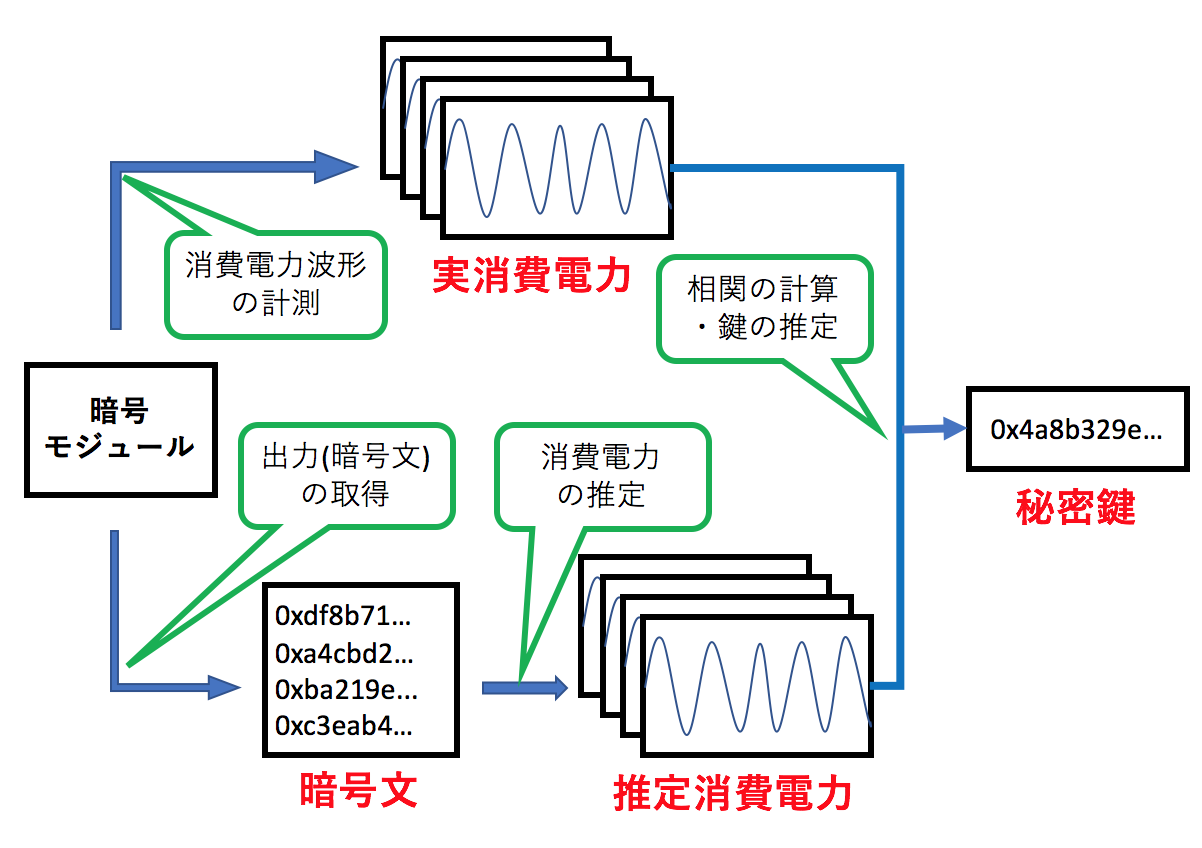
\includegraphics[width=\hsize, bb=0 0 600 450]{../images/CPA_image1.png}
		\caption{CPAの流れ(イメージ図)}
	\end{center}
\end{figure}

\subsection{消費電力の推定}
本節では取得した暗号文をから消費電力を推定する手法について説明する.
消費電力の推定はどの処理が消費電力が大きいと仮定するかによって推定値が異なる.
本研修では各ビットの値の書き換えが消費電力が大きいと仮定し,バイトごとの最終ラウンド前後の値のハミング距離 (Hamming Distance, HD値) を推定消費電力として使用する.
ハミング距離は取得した暗号文を仮定したラウンド鍵を使って書き戻し,暗号文自体との XOR をとることで求められる.
即ち,暗号文の特定のバイトをそれぞれ$c_x$,$c_y$とすると,

\begin{equation}
{\rm HD}_{x} = {\rm InvSbox(InvShiftRows(AddRoundKey}(c_{x}))) \oplus c_{y}
\end{equation}

\vspace{0.7cm}
ただし ShiftRows の処理によりバイトの位置がずれるため,
\underline{書き戻すバイトと XOR をとるバイトが異なる}点には十分に注意が必要
である.
推定消費電力は,暗号文の全バイト・全鍵値について上のように求めたHD値をテーブルとして扱う.
以後,このテーブルを\textbf{HDテーブル}と呼ぶ(図2).
HDテーブルは基本的に $(暗号文数) \times 16 \times 256$ の3次元テーブル,
または $(暗号文数) \times 4096$ の2次元テーブル
となる.

\newpage
\begin{figure}[htbp]
	\begin{center}
		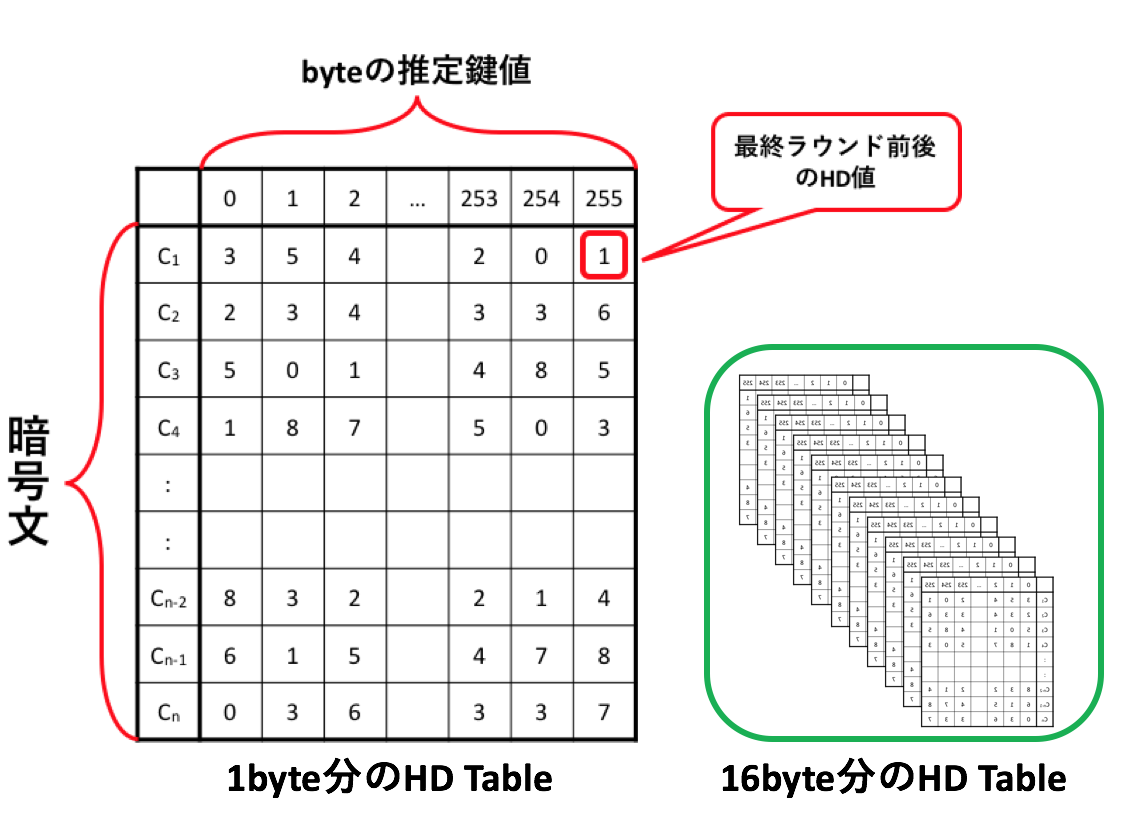
\includegraphics[width=0.8\hsize, bb=0 0 600 500]{../images/CPA_image2.png}
		\caption{HDテーブル}
	\end{center}
\end{figure}

\subsection{鍵値の推定}
本節では前節で推定したHDテーブルと計測した波形から鍵値を推定する手法について説明する.
本研修では計測した波形はcsv形式で保存されている.
作成したHDテーブルは値の書き換えを行う瞬間の消費電力を推定したものであるため,計測した波形からも値の書き換えが行われていると思われる時間を特定し値を抽出する必要がある.
相関係数の計算には\textbf{ピアソンの相関係数}を使用する.
各バイトで最も相関が大きくなったラウンド鍵の鍵値がそのバイトのラウンド鍵と推定できる.
ただし実際の攻撃を考える際は,波形によっては正しい鍵値でも相関係数が低くなるものや,正しい鍵値と誤った鍵値の相関係数がほとんど変わらないものも存在するため,鍵が推定できたと判断する基準については熟慮する必要がある.

\subsection{鍵の書き戻し}
AES において,ラウンド鍵は秘密鍵を拡張して生成する.
反対に,ラウンド鍵の値がわかればそこから一定の操作を行うことで元々の秘密鍵を求めることも可能である.したがって,ラウンド鍵を解析できることは秘密鍵を解析できることと同義として扱うことができる.
本書では鍵の書き戻しのアルゴリズムについては省略するが,比較的容易に書き戻せるため研修ではラウンド鍵を書き戻し秘密鍵の値まで求めることとする.

\newpage
\begin{figure}[htbp]
	\begin{center}
		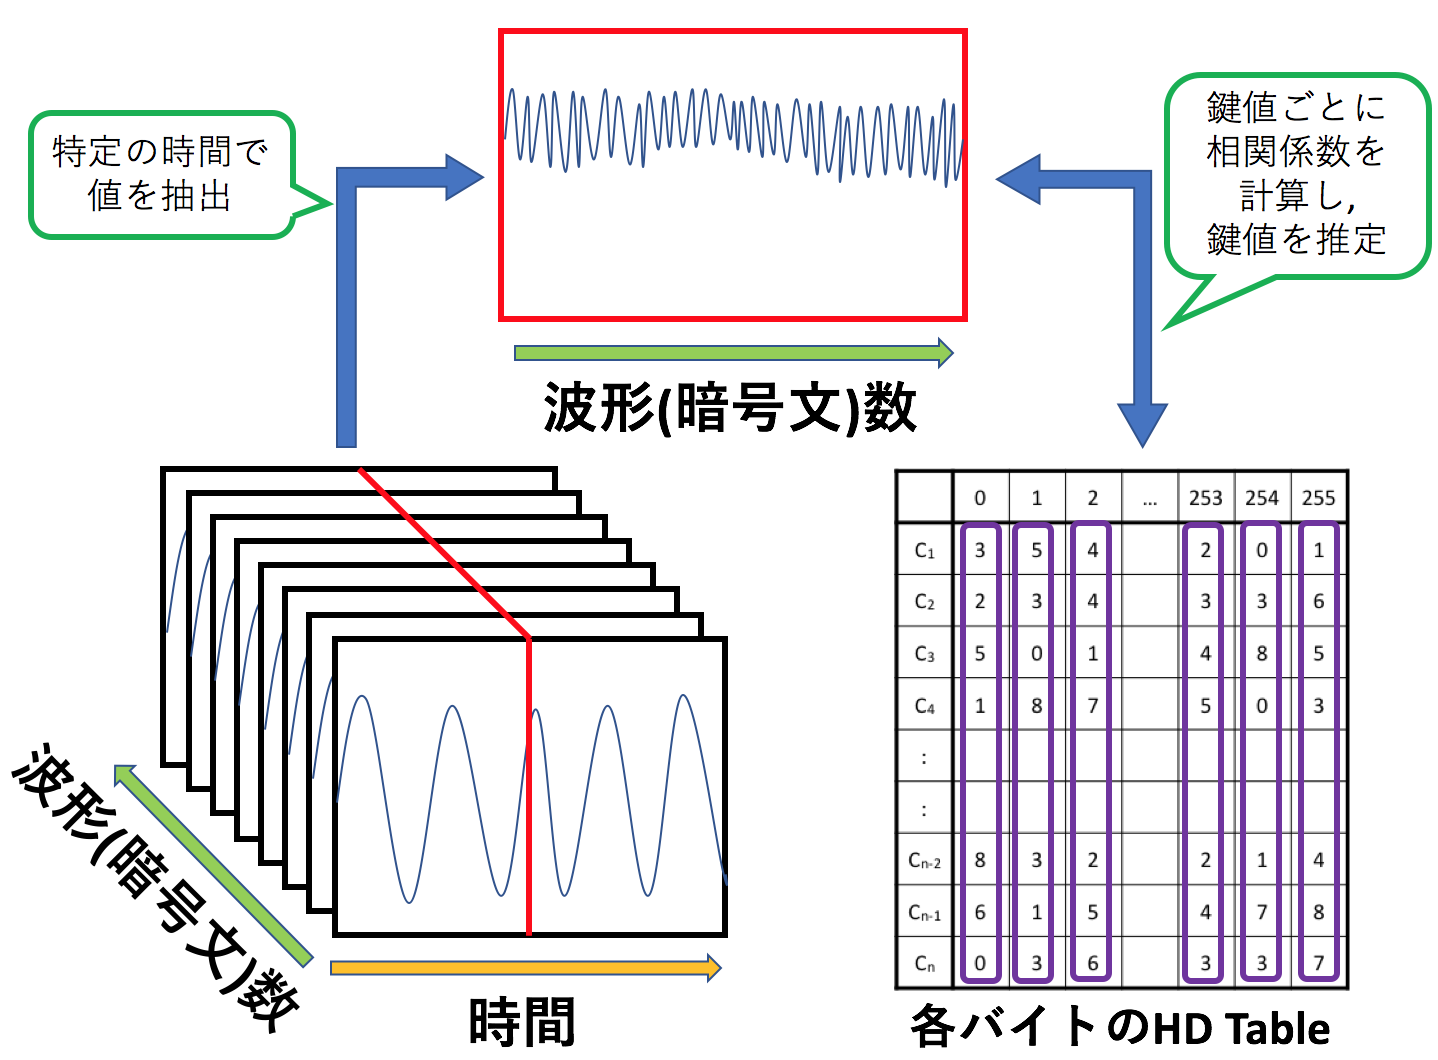
\includegraphics[width=0.8\hsize, bb=0 0 750 550]{../images/CPA_image3.png}
		\caption{鍵の推定}
	\end{center}
\end{figure}

\subsection{注意点・ヒント}
\begin{itemize}
\item CPAはより少ない波形数で鍵を解析することが目標となるため,プログラムを書く際には波形数を変更しやすいように書くと良い.
\item 使用する波形数に大きく左右されるが,プログラムの実行には数時間かかることも多いため,探索範囲はなるべく絞って探索を行うと良い.
\item HDテーブルの生成にも時間がかかるため,一度作成したらテキストファイルに書き込むなどしておいて2度目以降はファイルを読み込む方が効率良く試行できる.
\item 推定した鍵値が正しいかの判定法として,各鍵値の波形数に対する相関係数のグラフを用いると判断しやすくなる(ただし,プログラムの実行にかかる時間は長くなるため注意が必要).
\end{itemize}

\section{レポートについて}
練習の一環として本研修のレポートはTexにより作成するものとする.
記述したプログラム,推定された鍵値とその相関係数,簡単な考察を書くこと.

\begin{thebibliography}{99}
\bibitem{1} AES \url{nvlpubs.nist.gov/nistpubs/FIPS/NIST.FIPS.197.pdf}
\end{thebibliography}

\end{document}
